\section{Árbol de Soluciones}

\begin{figure}[H]
      \centering
      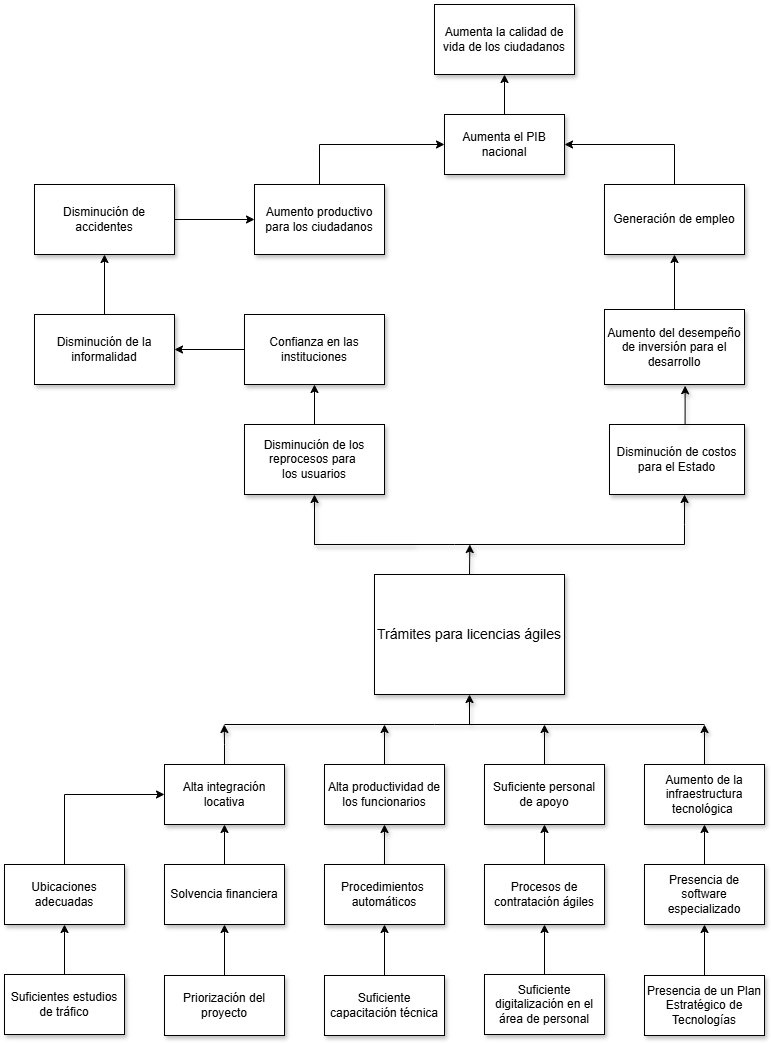
\includegraphics[width=0.9\linewidth]{formulacion/solutions-tree/img/Arbol_Soluciones.png}
      \caption{Árbol de Soluciones.}
      \label{fig:solutions_tree}
      \vspace{0.2cm}
      \small Fuente: Elaboración propia.
\end{figure}


\section{Actividades}
\label{sec:Actividades}

\subsection{Trámites para licencias ágiles}

\subsubsection{Diseño e implementación del sistema de trámites}
\begin{itemize}
  \item Definir requerimientos funcionales y no funcionales del sistema (RF y RNF).
  \item Diseñar la arquitectura, los módulos y el diagrama de componentes.
  \item Desarrollar el backend, frontend e integraciones (RUNT, CRC, pasarela de pagos).
  \item Ejecutar pruebas funcionales, de integración, rendimiento y seguridad.
  \item Preparar el despliegue en ambiente productivo y el plan de contingencia.
\end{itemize}

\subsubsection{Puesta en operación piloto}
\begin{itemize}
  \item Configurar parámetros de operación (horarios, tipos de trámite, sedes).
  \item Capacitar a operadores y supervisores en el uso del sistema.
  \item Ejecutar el piloto con monitoreo diario de tiempos de atención y reprocesos.
  \item Ajustar los flujos según las incidencias detectadas en el piloto.
\end{itemize}

\subsection{Alta integración locativa}

\subsubsection{Ubicaciones adecuadas}
\begin{itemize}
  \item Realizar diagnóstico de los espacios físicos actuales (capacidad, accesos, colas).
  \item Levantar el plano locativo y los flujos de usuarios y funcionarios.
  \item Definir criterios técnicos para la nueva disposición de áreas (zona de espera, ventanillas, archivo, supervisor).
  \item Socializar la propuesta con la Secretaría y obtener su aprobación.
\end{itemize}

\subsubsection{Suficientes estudios de tráfico}
\begin{itemize}
  \item Contratar o realizar un estudio de tráfico y demanda por franja horaria.
  \item Analizar tiempos de desplazamiento y accesibilidad (transporte público, parqueaderos).
  \item Incorporar los resultados del estudio en la reestructuración de áreas y horarios de atención.
\end{itemize}

\subsubsection{Solvencia financiera}
\begin{itemize}
  \item Formular el proyecto de inversión locativa (costos de obra, mobiliario y TI).
  \item Incluir el proyecto en el plan de inversiones de la Secretaría o del municipio.
  \item Gestionar la aprobación presupuestal y las fuentes de financiación.
\end{itemize}

\subsubsection{Priorización del proyecto}
\begin{itemize}
  \item Justificar el proyecto con indicadores de reprocesos, tiempos de atención y quejas.
  \item Presentar el proyecto en los comités de planeación y modernización institucional.
  \item Asegurar su inclusión prioritaria en el plan de acción anual.
\end{itemize}

\subsection{Alta productividad de los funcionarios}

\subsubsection{Procedimientos automáticos}
\begin{itemize}
  \item Identificar procesos susceptibles de automatización usando RF y casos de uso.
  \item Diseñar flujos automatizados mediante diagramas de actividades.
  \item Implementar los módulos correspondientes (gestión de llegada, verificación documental, conciliación de pagos, auditoría).
  \item Ejecutar pruebas y capacitación focalizada en los nuevos flujos.
\end{itemize}

\subsubsection{Suficiente capacitación técnica}
\begin{itemize}
  \item Elaborar un plan de capacitación en herramientas digitales y en el sistema de licencias.
  \item Desarrollar materiales de apoyo (manuales, videos y guías rápidas).
  \item Programar sesiones de capacitación por rol.
  \item Evaluar el aprendizaje mediante ejercicios prácticos y métricas de desempeño antes y después.
\end{itemize}

\subsubsection{Programas de bienestar y desempeño}
\begin{itemize}
  \item Implementar un programa de bienestar laboral ligado al SG-SST.
  \item Establecer indicadores individuales de productividad.
  \item Realizar evaluaciones periódicas de desempeño con retroalimentación.
\end{itemize}

\subsection{Suficiente personal de apoyo}

\subsubsection{Reclutamiento de personal administrativo y técnico}
\begin{itemize}
  \item Determinar las necesidades de personal según el estudio de cargas y la proyección de demanda.
  \item Definir perfiles y responsabilidades.
  \item Ejecutar procesos de selección mediante convocatorias, entrevistas y pruebas técnicas.
\end{itemize}

\subsubsection{Capacitación inicial}
\begin{itemize}
  \item Diseñar una inducción específica para el nuevo personal.
  \item Realizar sesiones de acompañamiento en sitio durante las primeras semanas.
\end{itemize}

\subsubsection{Definición de roles y turnos}
\begin{itemize}
  \item Establecer turnos rotativos y cobertura mínima por franja horaria.
  \item Configurar el sistema de gestión de usuarios y permisos.
  \item Documentar la matriz de roles, permisos y responsabilidades.
\end{itemize}

\subsubsection{Evaluación de desempeño del personal de apoyo}
\begin{itemize}
  \item Medir tiempos de atención y calidad del registro en el sistema.
  \item Aplicar encuestas de satisfacción al ciudadano.
  \item Definir planes de mejora o reentrenamiento según los resultados.
\end{itemize}

\subsection{Aumento de la infraestructura tecnológica}

\subsubsection{Compra de servidores y equipos e infraestructura en la nube}
\begin{itemize}
  \item Definir especificaciones técnicas según los RNF.
  \item Adquirir equipos de usuario y dispositivos especializados.
  \item Contratar servicios en la nube según los lineamientos vigentes.
\end{itemize}

\subsubsection{Modernización del centro de datos y servicios}
\begin{itemize}
  \item Configurar ambientes de desarrollo, pruebas y producción.
  \item Implementar políticas de monitoreo, respaldos y redundancia.
\end{itemize}

\subsubsection{Migración a la nube}
\begin{itemize}
  \item Planear la migración de datos y servicios con estrategia de reversa.
  \item Ejecutar la migración controlada y las pruebas posteriores.
\end{itemize}

\subsubsection{Implementación de ciberseguridad}
\begin{itemize}
  \item Definir e implementar controles del SGSI.
  \item Configurar autenticación fuerte, auditoría y gestión de incidentes.
\end{itemize}

\subsubsection{Presencia de software especializado}
\begin{itemize}
  \item Seleccionar o desarrollar una solución especializada para el trámite de licencias.
  \item Integrar los módulos del sistema.
  \item Mantener control de versiones, pruebas automatizadas y documentación técnica.
\end{itemize}

\subsection{Efectos intermedios y finales del árbol}

\subsubsection{Disminución de los reprocesos para los usuarios}
\begin{itemize}
  \item Configurar el módulo de gestión de excepciones y reprocesos con SLA definidos.
  \item Analizar mensualmente las causas de reproceso y ajustar las reglas de negocio.
\end{itemize}

\subsubsection{Confianza en las instituciones}
\begin{itemize}
  \item Implementar notificaciones y un portal ciudadano para la trazabilidad del trámite.
  \item Publicar indicadores de desempeño y tiempos de atención.
\end{itemize}

\subsubsection{Disminución de la informalidad y de accidentes}
\begin{itemize}
  \item Cruzar datos de licencias emitidas con estadísticas de siniestros y sanciones.
  \item Diseñar campañas pedagógicas basadas en la información del sistema.
\end{itemize}

\subsubsection{Aumento productivo para los ciudadanos y el PIB}
\begin{itemize}
  \item Medir la reducción del tiempo promedio del trámite.
  \item Analizar el impacto en empleo formal y productividad.
\end{itemize}

\subsubsection{Disminución de costos para el Estado y mejora del desempeño de la inversión}
\begin{itemize}
  \item Comparar los costos operativos antes y después de la automatización.
  \item Utilizar estas métricas para justificar nuevas inversiones y escalar el piloto.
\end{itemize}

